\section{Why don't we understand the news?}

The day the result of the 2016 United Kingdom EU Membership Referendum was announced, the Google Trends Twitter account reported a 250\% increase in searches for ``What happens if we leave the EU?'' \citep{googletrends}. Much like the case of David Leonhardt's article for the New York Times in 2008 which began, ``Raise your hand if you don't quite understand this whole financial crisis,'' national news commentary had focused on little else in the preceding months. It has become apparent that prolific coverage alone is not enough to engage and support the public in understanding current events.

Historically, news media has been limited in the volume of content it can produce by physical constraints such as printing costs, but the rise of the internet as a platform to deliver it has lead to an explosion of content, both through existing media channels and through competing social media websites and blogs. The term \textit{ambient news} was coined by Hargreaves and Thomas \citep{newnewsoldnews} to describe the ubiquity of news in the current information landscape. Others have commented in a more critical light; describing the proliferation of competing news media as ``as pervasive--and in some ways as invasive--as advertising.'' \citep[p.2]{overloadjournalismsbattle}


In 2007, The Associated Press conducted an extensive field study \citep{anewmodelfornews} into the news consumption habits of young adults. Among their key findings were three points which essentially summarise the news overload issue;
\begin{itemize}
	\item \textbf{``Consumers are experiencing news fatigue.''} \par
	The study found participants were debilitated, and that their levels of dissatisfaction lead to a decrease in the effort they put into news acquisition. This is consistent with multiple other studies \citep{newsandtheoverloadedcustomer, UnderstandingTheParticipatoryNewsConsumer, InformationAccessinComplexPoorlyStructuredInformationSpaces} which found participants across every demographic were overwhelmed by the amount of news content available to them and agreed it prevented them exploring news on less familiar topics. 
	
	\item \textbf{``Story resolution is key.''} \par
	Participants' consistent enjoyment of sports and entertainment news was due in part to the formulaic storytelling which characterises these types of journalism, with clear chronology to provide contextual back story. The feeling of enjoyment gained from reading procedural stories directly contrasts with what the same participants experienced reading World news, where they struggled to find resolution to stories which were unfolding at the time.
	
	\item \textbf{``Consumers want depth but aren't getting it''} \par
	It was observed that participants, in their efforts to discover \textit{below-the-fold} content (defined in the context of the AP's model \citep[p.37]{anewmodelfornews}) from particular headlines, often found themselves reading the same summary-level content from different news sources. A recommendation was made that news providers should be``designing innovative formats and creating easier pathways to deep content'' \citep[p.49]{anewmodelfornews} in order to support this.
\end{itemize}

Initially, the third point seems to be a direct contradiction to the first; we are overwhelmed by the volume of news we are exposed to, but we also crave more detail from the news we do consume. However, it brings to light the issue of information \textit{quality} as a requirement of news consumers.

 Journalism, and therefore its quality, can be viewed along a spectrum between two models; a model for the communication of facts, and a model for entertainment and storytelling. From the three points above, it is clear that quality at both ends of the spectrum is being sought, since the desire for quality below-the-fold content is covered by the first model, and the desire for quality story resolution by the second.

\subsection{Information Overload}

News fatigue is a domain-specific type of information overload, a phenomenon formally defined as ``when the information processing demands on time to perform interactions and internal calculations exceed the supply or capacity of time available for such processing.'' \citep[p.206]{InformationOverloadATemporalApproach} Information overload is a multifaceted problem which can be modelled as a combination of three contributing factors (Figure \ref{fig:dimensions}).

\begin{figure}[htbp!]
	\centering
	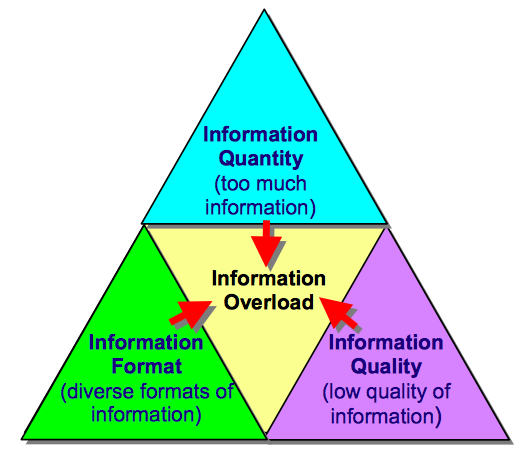
\includegraphics[width=.55\textwidth]{img/lit-survey/overload-model.png}
	\caption{Dimensions of information overload, as defined by Ho and Tang \citep{TowardsAnOptimalResolutionToInformationOverload}.}
	\label{fig:dimensions}
\end{figure}

These factors correspond directly to the three points previously identified from the Associated Press study \citep{anewmodelfornews}. Information quantity causes news fatigue, information format determines the level of possible story resolution, and information quality determines how much depth a reader can gain from the news they consume. The authors did not find a single solution which could address all three factors, but they did identify information quantity as the most significant contributor to overload.

Bergamaschi et al.\citep{GuestEditorsIntroductionInformationOverload} further decomposed information quantity into spatial and temporal dimensions in the specific context of news articles. Spatial quantity refers to articles which are near-identical in terms of facts presented being published by different media outlets, and temporal quantity refers to articles on a single topic being published and updated in quick succession over a short period of time.

To adequately address news fatigue, all four dimensions of information overload should be considered, and will therefore be explored in more detail.

\subsubsection{Information Quality}
In the context of factual data rather than news specifically, Strong et al \citep{DataQualityInContext} defined information quality in terms of four components; intrinsic quality, accessibility quality, contextual quality and representational quality. If news can be rationalised to its core function as an interpretation of facts and other raw data such as images, then this same framework can be experimentally applied to news journalism in order to determine which factors could influence its quality.

Intrinsic quality is a measure of the accuracy, objectivity, believability and reputation of data. In the context of news, the first three factors would typically be true for all major news sources, and the reputation would be dependent on whether the article originated from a trusted source or not. Accessibility quality is less relevant to online news media, as it is concerned with data access and security. Contextual quality is the most relevant category in respect to news, concerning timeliness, amount of data, and value-added. In the news domain, this would mean an article's quality is dependent on its performance against a background of other articles; whether or not it contributes anything recent or previously unknown. Finally, representational quality is concerned with ease of understanding and interpretability, which are easily translatable concepts.

To summarise, applying the Information Quality Framework\citep{DataQualityInContext} to news articles suggest quality can be influenced by the reputation of the source, the timeliness of publication, value-added by the article (i.e. content which couldn't be derived from other sources) and ease of understanding.


\subsubsection{Information Format}
The domain of news articles is a more specific information space than that of documents in general, and by nature most news articles share some common formatting and structural elements such as headlines, timestamps, and relevant images. As a result of this, it is unlikely that any two articles from popular news providers would be diverse enough in content format to overshadow the information quantity problem.
%News aggregators, such as Google News\footnote{http://news.google.co.uk} address differences in visual formatting of sources by extracting images, headlines and sub-headlines consistently irrespective of source.

\subsubsection{Temporal Quantity}

The rise of social media sites such as Twitter delivering news to consumers has lead to a high degree of news fragmentation, due to the constraints of the microblogging service's 140-character limit. 24-hour television news paved the way for new formats of real-time content delivery, and the ever-expanding network of online social media channels stepped up to deliver. It logically follows from the fragmented nature of real-time news journalism that temporal quality suffers; stories are published and updated intermittently over short periods of time, meaning there is more for the consumer to piece together to understand a story.

The fragmentation is somewhat mitigated by Twitter's use of hashtags to denote a Tweet's topics. Hashtags help readers form a coherent and picture of unfolding events from the incremental contributions of thousands of participating users. \citep{BlogsTwitterAndBreakingNews}


Murata and Phuvipadawat \citep{BreakingNewsDetectionAndTrackingInTwitter} developed a methodology to collect and group Tweets on breaking news topics, using hashtags for topic identification or \textit{story-finding}, and grouping similar messages together to form a single news story. Their algorithm for similarity is a function of the TF-IDF \citep{IntroductionToInformationRetrieval} of the two messages and the number of named entities they have in common.

\subsubsection{Spatial Quantity}
It is in the nature of news that newsworthy stories get repeated across multiple sources. When consumers read news on a particular from more than once source, it is likely that they will read variations on the same facts in multiple articles.

Attempts such as \citep{InformationFusionInTheContextOfMultiDocumentSummarization} have been made to synthesise summaries of collections of similar online documents, a practice here termed \textit{information fusion}, with news articles from different sources being given as a specific use-case. However, the process of extracting common sentences between documents was in order to reformulate them into a single summary, rather than to determine the level of similarity between the documents.

A more relevant approach was presented in \citep{UtilizingPhraseSimilarityMeasures}, where the \textit{title} and \textit{description} attributes of elements in RSS feeds were used as content descriptors to mitigate the overhead of processing entire documents for phrases. This decision can be supported by other work such as \citep{IdentifyingTopicsByPosition}, which found up to 50\% of a news document's keywords can be found in its title. The content descriptors are then used to compute phrase \textit{n}-grams as a measure of similarity between any two documents. The similarities in this case were used to remove subsumed articles and cluster non-redundant similar ones, in order to streamline feed content for readers.

It should be noted that there is an overlap between the notion of spacial quantity and one of the influencing factors in information quality; contextual quality. If a feed contains two articles which state the same number of identical facts, they therefore contribute to information overload on both the qualitative and quantitative fronts.


\subsection{Supporting Sensemaking}

Sensemaking is the basis for forming contextual knowledge; the process by which we incorporate new information into our existing cognitive frameworks, and how we go from reading something to understanding it. \citep{FromInformationToKnowing} In broader terms, Weick et al. describe sensemaking as ``[being] about the question: What does an event mean? In the context of everyday life, when people confront something unintelligible and ask, `What’s the story here?'{}'' \citep[p.85]{OrganizingAndTheProcessOfSensemaking} This relates directly to the news overload problem because sensemaking describes the contextual story resolution that the Associated Press study \citep{anewmodelfornews} identified news consumers are craving.

Offering further insight into Leonhard's aforementioned New York Times article during the financial crisis, Journalism Professor Jay Rosen wrote in a blog post some months after the article was published, ``there are certain very important stories -- and the mortgage crisis is a good example -- where until I grasp the whole I am unable to make sense of any part.''\citep{NationalExplainer} 

It has also been observed that often readers are not interested in specific articles on a subject, and only the thematic content of the topic they belong to.\citep{AnalysingUserAccessToAnOnlineNewspaper} How then, do readers make sense of a collection of articles surrounding a particular topic?

When presented with a large document collection on any kind, people typically start by clustering the contents into groups which form a heuristic representation or mental model which can be used to provide an overview. \citep{BeingLiteratreWithLargeDocumentCollections}

Writing for the Columbia Journalism review in 2008, Nordenson outlined a suggestion for the new roles of journalism in the information era; ``By linking stories to one another and to background information and analysis, news organizations help news consumers find their way through a flood of information that without such mediation could be overwhelming and nearly meaningless.''\citep[p.10]{overloadjournalismsbattle} 

Similarly, \citep{FromInformationToKnowing} makes the recommendation in the context of contemporary media consumption that news providers should adapt to an environment of news overload by adding facilities enabling readers to categorise, sort and search news collections. Additional findings of this study suggested that the contextual background provided by having more detailed coverage aids the sensemaking process, as it helps users form links between new information and their existing frameworks, but this presents an interesting conflict with the goal of reducing information overload.

A recognised technique for bridging the gap between a set of data and a user's mental model and subsequent of the data is information visualisation, or InfoVis. \citep{UnderstandingAndCharacterizingInsights, ThemeRiver}.

Yi et al. \citep{UnderstandingAndCharacterizingInsights} identified four overlapping InfoVis processes which describe how insight can be gained after sensemaking; \textit{Provide Overview}, \textit{Adjust}, \textit{Detect Pattern}, and \textit{Match Mental Model}. The Provide Overview process allows a reader to recognise what they know and what they don't know from the information they are processing. Adjusting allows them to change the level of abstraction or field of selection of that information. The Detect Pattern procedure is where structure and trends are found, whether expected or otherwise. Match Mental Model is where the links are formed between the new data and the users' existing cognitive frameworks.

Even though the structure and purpose news documents does not naturally suggest an appropriate visualisation for them, it is still the case that visualisation of non-spatial data can provide vital insight, especially when the quantity of data is vast. ``Because we live and perceive in a physical world, it is easier to convey the information to the observer if the information is represented by being mapped to the familiar physical space.''\citep[p.39]{VisualizationsNewTack}


\section{Designing Visualisations}

\subsection{Keyword Extraction}
%30\% of keywords are inferred rather than mentioned directly in text \citep{IdentifyingTopicsByPosition}

\subsection{Topic Coverage}

\subsection{Maps}

\section{Evaluating Usefulness}



\section{Conclusions}